\subsection{Thorによる実装}
手法のところで概観した通り,thorを用いることで記述の簡略化が期待できる.ここでは,実際に書き換える前後,すなわちoptparse版とthor版の対応するコードを比較することで,以下の具体的な違い

\begin{itemize}
\item クラス初期化
\item コマンド定義
\item CLIの実行プロセス
\end{itemize}
について詳しく検討を行う.

\subsubsection{クラス初期化}
\begin{figure}[htbp]\begin{center}
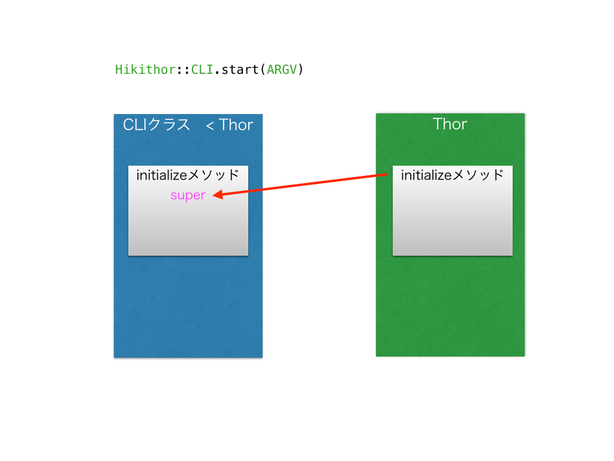
\includegraphics[width=6cm,bb=0 0 442 432]{../figs/./hikiutils_yamane.003.jpg}
\caption{Thorのinitializeでのコード}
\label{default}\end{center}\end{figure}
Thorのinitializeでのコードはつぎの通りである.

\begin{enumerate}
\item Hikithor::CLI.start(ARGV)が呼ばれる
\item initializeメソッドが呼ばれる
\item これではThorのinitializeメソッドが呼ばれない
\item superを書くことでThorのinitializeメソッドが呼ばれる
\end{enumerate}
optparseではrequireでoptparseを呼びoptparseのinitializeを定義する必要はないが,Thorはinitializeを定義する必要がある.Thorの定義方法はrequireでThorを呼びCLIクラスで継承し,initializeメソッドにsuperを書くことでThorのinitializeが呼ばれる.initializeメソッド内ではThorの初期設定がされていないため,スーパークラスのメソッドを読み出してくれるsuperを書き加えることで図のようにinitializeメソッド内でThorのinitilalizeメソッドが呼ばれ定義される.
\begin{lstlisting}[style=customRuby]

module Hikithor

  DATA_FILE=File.join(ENV['HOME'],'.hikirc')
  attr_accessor :src, :target, :editor_command, :browser, :data_name, :l_dir

  class CLI < Thor
   def initialize(*args)
      super
      @data_name=['nick_name','local_dir','local_uri','global_dir','global_uri']
      data_path = File.join(ENV['HOME'], '.hikirc')
      DataFiles.prepare(data_path)

      ...以下略...
   end
\end{lstlisting}
\subsubsection{コマンド定義}
\begin{figure}[htbp]\begin{center}
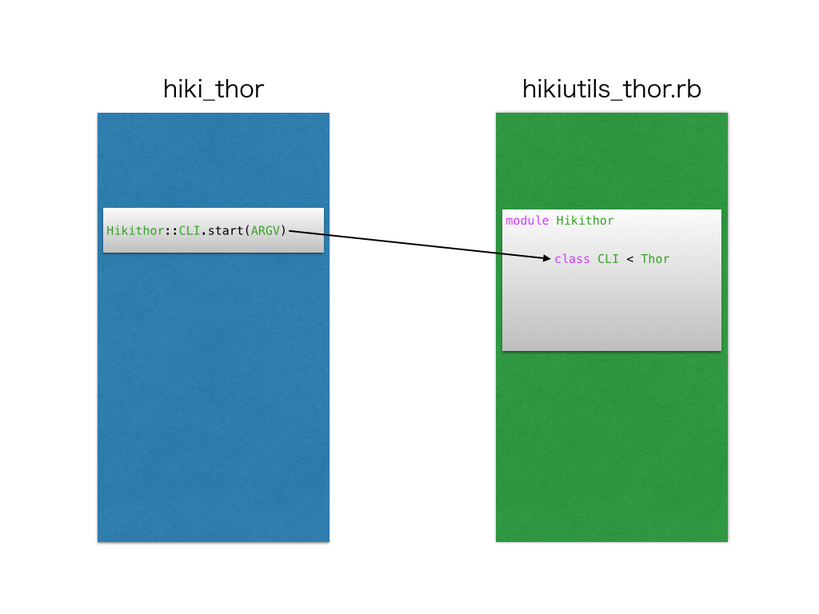
\includegraphics[width=6cm,bb=0 0 442 432]{../figs/./hikiutils_yamane.004.jpg}
\caption{thorにおけるコマンド記述のひな形.}
\label{default}\end{center}\end{figure}
thorではoptparseのような登録処理はない.図にある通りにコマンドが記述され,それらは以下のように構成される.

\begin{enumerate}
\item desc以降にコマンド名と,その説明が記述される.これらはコマンドhelpで一覧として表示させる
\item mapによって別のコマンド名でも実行できるように定義される.
\item defで定義されたメソッドの実行コード
\end{enumerate}
Thorではdescで一覧を表示されるコマンド名,コマンドの説明を登録する.しかし,ここで記述したコマンドは単に一覧で表示させるためのものであり,実際に実行される時に呼び出すコマンド名は,defで定義された名前である.Thorでは処理実行を行うメソッド名がコマンド名となり,コマンド名1つが対応する.

これに別名を与えるために利用されるキーワードがmapである.
\begin{quote}\begin{verbatim}
map A => B
\end{verbatim}\end{quote}
mapとはBと呼ばれるメソッドをAでも呼べるようにしてくれるものである.
よって,これを使うことでコマンドの別名を指定することができる.
\begin{lstlisting}[style=customRuby]
    desc 'show,--show', 'show sources'
    map "--show" => "show"
    def show
      printf("target_no:%i\n",@src[:target])
      printf("editor_command:%s\n",@src[:editor_command])
      ,,,以下略...
    end
\end{lstlisting}
以上より,Thorではコマンドの指定と処理にはdesc,map,処理メソッドだけで済む.optparseではコマンドを登録するためのメソッドと処理メソッドの両方が必要になっていた.一方Thorでは,処理メソッドが直接コマンド名となるため記述が簡潔になる.

\subsubsection{CLIの実行プロセス}
\begin{figure}[htbp]\begin{center}
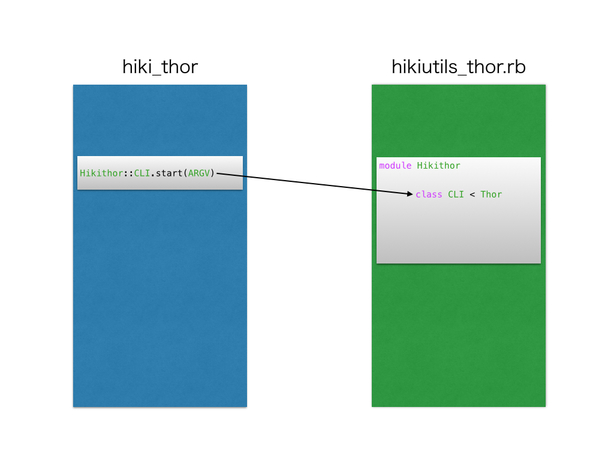
\includegraphics[width=6cm,bb=0 0 442 432]{../figs/./hikiutils_yamane.006.jpg}
\caption{CLIの実行プロセス.}
\label{default}\end{center}\end{figure}
Thorにおけるcliの実行プロセスは次の通りである.

\begin{enumerate}
\item hiki\_thorのHikithor::CLI.start(ARGV)でhikiutils\_thor.rbのCLIクラスを呼ぶ
\item hikiutils\_thor.rbのCLIクラスのメソッドを順に実行していく
\end{enumerate}
Thorではstart(ARGV)を呼び出すことでCLIを開始する.Hikithor::CLI.start(ARGV)を実行されることによりrequireで呼ばれているhikiutils\_thor.rbのCLIコマンドを順に実行する.そして,入力されたコマンドと一致するメソッドを探し,そのコマンドの処理が実行される.
\begin{lstlisting}[style=customRuby]
#!/usr/bin/env ruby                                                             

require "hikiutils_thor"

Hikithor::CLI.start(ARGV)
\end{lstlisting}\begin{quote}\begin{verbatim}

module Hikithor

  DATA_FILE=File.join(ENV['HOME'],'.hikirc')
  attr_accessor :src, :target, :editor_command, :browser, :data_name, :l_dir

  class CLI < Thor
   def initialize(*args)
      super
      @data_name=['nick_name','local_dir','local_uri','global_dir','global_uri']
      data_path = File.join(ENV['HOME'], '.hikirc')
      DataFiles.prepare(data_path)
      ...以下略...
\end{verbatim}\end{quote}
Thorではクラスのメソッドを順に実行していくためrunメソッドとexecuteメソッドは必要ない.また,optparseでの実行手順はメソッドの移動回数が多く複雑であるが,Thorは単純で分かりやすいものとなっている.

\subsubsection{optparseとの全体的な比較}
コードからもThorのほうが短くなっていることが分かる.よって,Thorとoptparseでのコードの違いは以上の部分になるが全体的にもThorのほうがコードが短くなり,コマンドの定義も簡単に行うことができる.また,実行手順も分かりやすくコードが読みやすいため書き換えもすぐ行うことができるので,より直感的なコマンドを実装することも可能となった.

